\documentclass[letter, 10pt]{article}
\usepackage[utf8]{inputenc}
\usepackage[spanish]{babel}
\usepackage{amsfonts}
\usepackage{amsmath}
\usepackage{subfig}
\usepackage{graphicx}
\graphicspath{ {images/} }
\usepackage{url}
\usepackage[top=3cm,bottom=3cm,left=3.5cm,right=3.5cm,footskip=1.5cm,headheight=1.5cm,headsep=.5cm,textheight=3cm]{geometry}


\begin{document}
\title{Inteligencia Artificial \\ \begin{Large}Estado del Arte: Progressive Party Problem\end{Large}}
\author{[Roberto Fuentes Zenteno]}
\date{\today}
\maketitle


%--------------------No borrar esta secci\'on--------------------------------%
\section*{Evaluaci\'on}

\begin{tabular}{ll}
Resumen (5\%): & \underline{\hspace{2cm}} \\
Introducci\'on (5\%):  & \underline{\hspace{2cm}} \\
Definici\'on del Problema (10\%):  & \underline{\hspace{2cm}} \\
Estado del Arte (35\%):  & \underline{\hspace{2cm}} \\
Modelo Matem\'atico (20\%): &  \underline{\hspace{2cm}}\\
Conclusiones (20\%): &  \underline{\hspace{2cm}}\\
Bibliograf\'ia (5\%): & \underline{\hspace{2cm}}\\
 &  \\
\textbf{Nota Final (100\%)}:   & \underline{\hspace{2cm}}
\end{tabular}
%---------------------------------------------------------------------------%
\vspace{2cm}


\begin{abstract}
Se presenta el problema \textit{Progressive Party Problem} (PPP), propuesto por Peter Hubbard (\textit{Southampton
University}). Consiste en organizar de la mejor manera una ``fiesta progresiva'' en un grupo de yates, en donde durante periodos consecutivos de tiempo la tripulación de los yates invitados debe visitar los yates anfitriones. El objetivo del problema es asignar todas las tripulaciones visitantes a los yates anfitriones para cada período de tiempo, minimizando la cantidad de yates anfitriones. Se describe el problema, luego se analiza el estado actual del problema mediante el estado del arte, seguido de un modelo matemático, además de las técnicas que se han usado para abordarlo y los resultados acotados que se han obtenido. 
\textbf{Keywords}: PPP, optimización combinatoria, programación lineal entera, programación de restricciones,busqueda local.
\end{abstract}

\section{Introducción}
Una conferencia es una manera excelente en que las personas que tienen intereses comunes pueden reunirse e intercambiar las ideas m\'as vanguardistas de su campo. Es por esto que la gestión de eventos progresivos es un elemento importante a controlar y mejorar. En este documento, se presenta el \textit{Progressive Party Problem} (PPP), problema especifico que plante\'o Peter Hubbard, miembro de asociación \textit{Sea Wych Owners} y del departamento de matematicas de \textit{Southampton University} en el a\~no 1996~\cite{Kalvelagen20031713}, cuyo objetivo es asignar todas las tripulaciones visitantes a los yates anfitriones para cada período de tiempo, minimizando la cantidad de yates anfitriones. El documento proporciona el planteamiento del problema bien definido junto con su formulación a través de Programación entera y Programación de restricciones junto a una explicación de como fueron los resultados de ambos experimentos. Además, existen otros documentos donde se entrega la data del problema y sus respectivas soluciones usando distintas técnicas.
\\

\textit{Progressive Party Problem} (PPP) busca encontrar la mejor manera de gestionar yates invitados y anfitriones, donde los yates invitados podrán invitar a los anfitriones en determinados periodos de tiempo. Su objetivo es minimizar los yates anfitriones respetando ciertas restricciones, como evitar exceder la cantidad de los yates anfitriones o que las tripulaciones invitadas no podrán toparse más de una vez.
\\

La motivación del problema surge debido al problema originado en \textit{Bembridge}, Isla de \textit{Wight}~\cite{Kalvelagen20031713}. Su contexto es organizar un programa social para un paseo de yates, donde estos estaban amarrados en un puerto deportivo. Para que las personas se reúnan con tantos otros asistentes como le fuera posible, se planeó una fiesta nocturna en donde algunos de estos yates serian designados como anfitriones, y las tripulaciones de los barcos restantes ir\'ian visitando a estos yates anfitriones durante seis horas en periodos de media hora. El problema que enfrentaba el organizador del paseo era el de minimizar el número de los barcos anfitriones, ya que cada anfitrión tenía que ser abastecido con alimentos y otros prerrequisitos. 
\\

La estructura del actual trabajo es la siguiente: En la sección siguiente se define y se explica detalladamente el problema \textit{Progressive Party Problem}, en la sección 3 se plantea el estado del arte del problema analizado, indicando los soluciones encontradas hasta el d´ıa de hoy. Luego en la sección 4 se presenta el modelo matemático que mejor resuelve el problema con el fin de que cualquier persona sea capaz de interpretarlo. Finalmente en la sección 5 se concluye sobre el problema estudiado.

\section{Definición del Problema}
\subsection{Progressive Party Problem}
\subsubsection{Definición}
\textit{Progressive Party Problem} (PPP) busca encontrar la mejor manera de gestionar yates invitados y anfitriones, donde los yates invitados podrán invitar a los anfitriones en determinados periodos de tiempo. 

\subsubsection{Objetivo}
El objetivo de PPP es asignar todas las tripulaciones visitantes a los yates anfitriones para cada período de tiempo, minimizando la cantidad de yates anfitriones.

\subsubsection{Parametros}
\textit{Progressive Party Problem} tiene los siguientes parámetros:

\begin{itemize}
\item $H$: Cantidad de yates.
\item $K_i$: Capacidad del yate $i$.
\item $T$: cantidad de períodos.
\item $c_i$: cantidad de tripulantes del yate $i$.
\item $H_i$: 1 si el yate $i$ es un anfitrión.
\item $G_{ikt}$ = 1 si el yate $k$ es un invitado del yate $i$ en el período $t$
\item $m_{klt}$ = 1 si el yate $k$ y $l$ se encuentran en el período $t$.
\end{itemize}

\subsubsection{Variables}
Algunas variables de PPP son las siguientes:

    \begin{itemize}
      \item $h_i$: 1 si el yate $i$ es un yate anfitrión.
      \item $x_{ikt}$: 1 si el yate $k$ es un invitado del bote $i$ en el periodo $t$.
    \end{itemize}

\subsubsection{Restricciones}
\begin{itemize}
\item Un yate solo podrá ser visitado si es un yate anfitrión.
\item La capacidad de los yates anfitriones no se puede exceder.
\item Cada tripulación debe siempre tener un anfitrión asociado o ser uno.
\item Una tripulación invitada no podrá visitar un yate anfitrión más de una vez.
\item Las tripulaciones invitadas no podrán toparse más de una vez.
\end{itemize}

\subsection{Otras variantes}
Tenemos varios problemas relacionados con la gestión de yates, los cuales buscan distintas maneras de resolver el problema: Como un CSP, minimizar la cantidad de yates anfitriones, maximizar la duración de la fiesta, definir diferentes restricciones del problema. Las variantes clasicas son:

\begin{enumerate}
    \item \textbf{PPP as CSP}: \\
    Ver si es factible o no realizar una fiesta con las características dadas. Lo que se busca es encontrar una instanciación de las variables que cumpla con las restricciones descritas del problema (y sin una función objetivo). ~\cite{Brailsford:1996:OSE:241748.241755}
    
     \item \textbf{Uncapacited CPP}:\\
     Otra de las variantes del \textit{Progressive Party Problem} es resolver el problema sin considerar la capacidad de los barcos. Si ignoramos las restricciones de capacidad, sólo un barco anfitrión puede acomodar cualquier número de barcos invitados por un período de tiempo. Durante más de un período de tiempo, podemos encontrar fácilmente un límite inferior en el número de anfitriones requeridos del argumento siguiente. Por lo anterior, para el caso particular de 42 botes en total, 7 serán anfitriones y 35 invitados.
     
     Si $g$ tripulaciones visitan al $host$ $i$ en el periodo 1, entonces debe haber por lo menos $g$ otros anfitriones para poder distribuirlos a todos en el siguiente período de tiempo (Los huéspedes no pueden visitar un anfitrión $i$ otra vez, y deben visitar los $g$ anfitriones  diferentes para no reunirse con otra tripulación nuevamente). De hecho, los $g + 1$ anfitriones requeridos podrían acomodar a las $g$ tripulaciones en el periodo 1 sin que estos se encuentren nuevamente en el periodo 2, dando $g(g + 1)$ equipos invitados en total.
Por más de 2 períodos de tiempo, $g (g + 1)$ es claramente un límite superior en el número de equipos invitados que g + 1 $hosts$ pueden acomodar. Por ejemplo, 6 anfitriones pueden acomodar en la mayoría de 30 barcos de la huésped; 7 anfitriones pueden acomodar como máximo 42. De hecho, estos límites pueden ser alcanzados (aún suponiendo que no hay limitaciones en las capacidades de los anfitriones, y siempre que el número de períodos de tiempo no sea mayor que el número de anfitriones, en cuyo caso se hace imposible que las tripulaciones de invitados no visiten el mismo anfitrión más de una vez), por lo que con 42 barcos en total, necesitamos 7 para ser los anfitriones (y por lo tanto 35 para ser invitados).

     El problema con este enfoque recae en la vida real, donde los yates poseen una capacidad máxima, por lo que este enfoque no es el mas indicado para resolver el problema, Ademas de que el numero necesario de anfitriones para esta variante es de minimo 13 anfitriones. ~\cite{Smith1996}

    \item \textbf{A Lower Bound}: \\ 
    Un límite inferior en el número de yates anfitriones necesarios (teniendo en cuenta las limitaciones de capacidad) se encontró mediante la programación lineal para relajar de forma considerable el problema. Esto simplemente requería que las tripulaciones invitadas tuvieran en cuenta la capacidad de reserva total de los barcos anfitriones durante un período de tiempo. Este límite se puede encontrar alternativamente a partir de un simple argumento: una condición necesaria para la viabilidad es que la capacidad total de los barcos de acogida mayor que el tamaño total de la tripulación de todos los barcos, por lo que el menor número de huéspedes que cumplen con esta condición se encuentra ordenando los barcos en orden descendente de capacidad total. Con esto, los primeros 13 barcos pueden acomodar a todas las tripulaciones; Los primeros 12 barcos no pueden. Esto sugiere que en general los barcos anfitriones deben ser elegidos en orden descendente de capacidad total (Se toma como una heurística).~\cite{Smith1996}

\end{enumerate}

\section{Estado del Arte}
Hoy en día los eventos o conferencias son excelentes maneras en que personas con intereses en común puedan reunirse e intercambiar ideas. Para poder gestionar de mejor manera estos eventos, podemos trabajar estos casos como problemas de planificación de tiempo (\textit{Scheduling Problem}), donde un caso particular es el \textit{Progressive Party Problem} (PPP). 

\begin{figure}[ht]
 \centering
  \subfloat[Fiesta de yates, \textit{Island of wight}]{
   \label{f:Fiesta yates}
    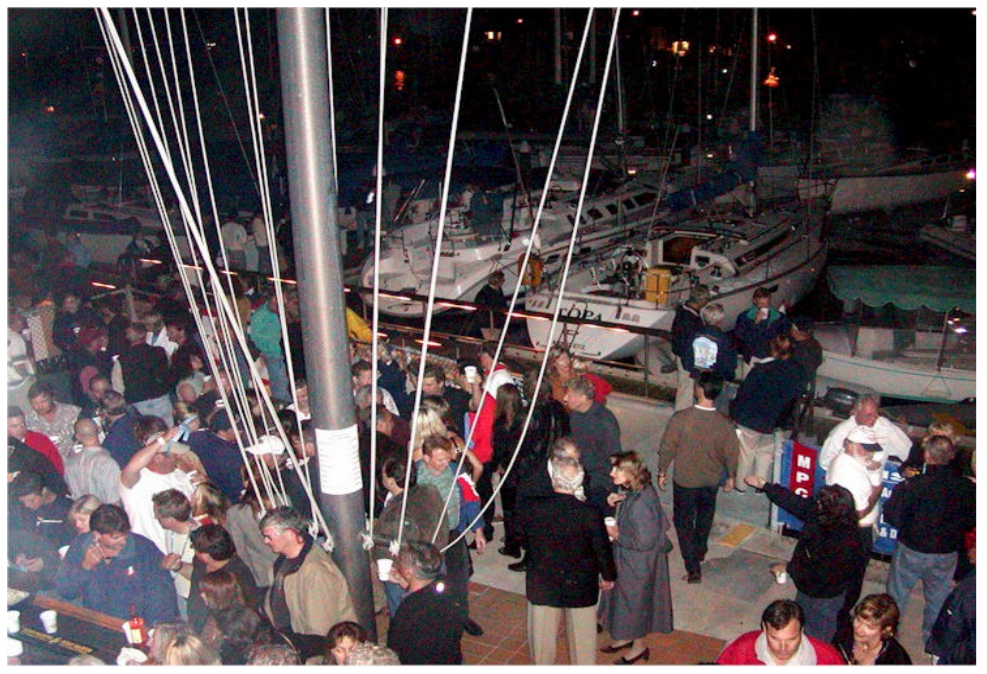
\includegraphics[width=0.5\textwidth]{party1.png}}
  \subfloat[Vista general de PPP]{
   \label{f:Vista general}
    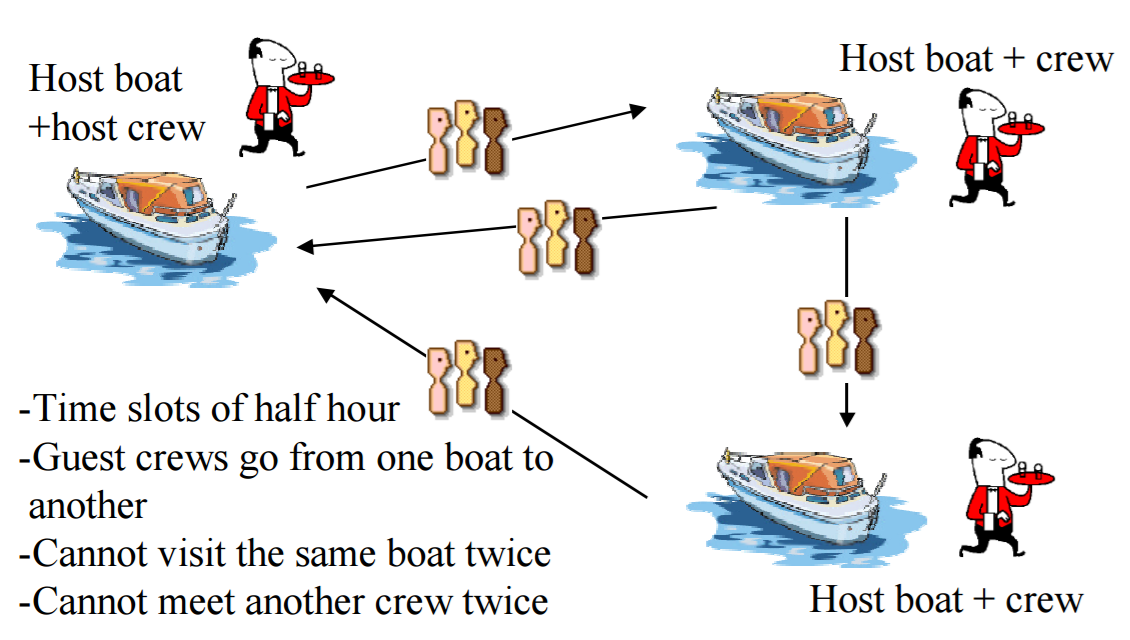
\includegraphics[width=0.5\textwidth]{party2.png}}
 \caption{Progressive Party Problem}
 \label{f:PPP}
\end{figure}

El problema fue originalmente propuesto por Peter Hubband de la Universidad de \textit{Southampton}, organizador de un club de yates con 42 botes y sus tripulaciones respectivas. Este importante evento nocturno tiene como objetivo organizar una fiesta donde cada tripulación socializa con tantas otras tripulaciones como le sea posible. El problema ahora es asignar todos los equipos invitados a los barcos anfitriones para cada uno de los intervalos de tiempo, utilizando el número mínimo de barcos anfitriones. Con el paso del tiempo, se van planteando más problemas con distintos objetivos referidos a la planificación de eventos, lo que da origen a todas las variantes que se mencionaron anteriormente. Es importante destacar que los primeros 3 yates serán yates anfitriones puesto que el primer yate es del organizador del evento, y los 2 siguientes contienen tripulaciones con niños. Las tripulaciones se separaron para que los padres permanecieran a bordo del
barco anfitrión y los niños se convirtieron en un "barco virtual" con capacidad cero. En conjunto con los niños del yate del organizador del evento se formaron tres barcos virtuales, sumando un total de 42 botes:

\begin{figure}[ht]
\centering
 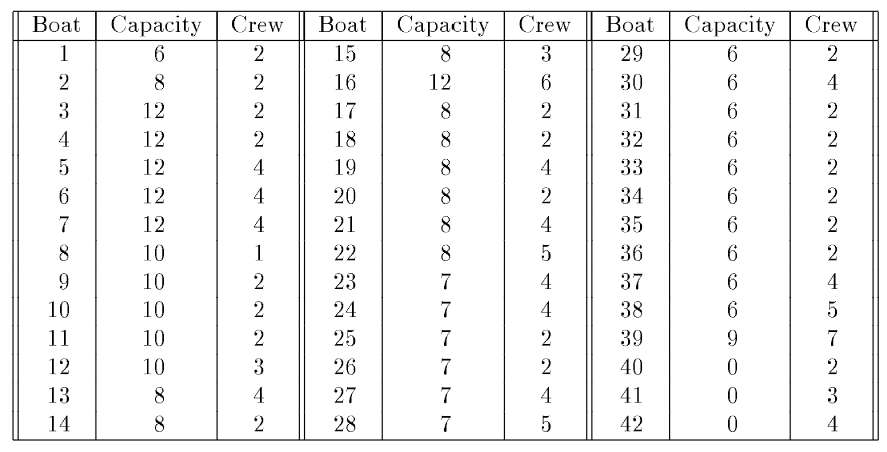
\includegraphics[width=1.0\textwidth]{party5.png}
 \caption{Data del problema real}
\end{figure}

En el paper \textit{The progressive party problem: Integer linear programming and constraint programming compared} ~\cite{Smith1996} se proponen dos tipos de modelos: a través de ILP (\textit{Integer-Linear Programming} ) y CP (\textit{Constraint Programming}). El documento nos habla de que a pesar de que ILP pareciera ser el método mas poderoso para resolver nuestro problema, a veces la programación de restricciones puede resolver estos problemas mas rápido. La formulación con programación lineal entera incluyendo todas las restricciones recae en un modelo muy largo. Probando varias estrategias nos damos cuenta de que lamentablemente todos los intentos de solución fallan. Por otra parte la programación de restricciones puede resolver este problema rápidamente, con un poco de ayuda manual. 

\begin{itemize}
\item \textbf{Enfoque con programación entera}
\begin{itemize}    
\item 
Luego de proponer el modelo con programación entera (el cual se muestra más adelante), se determino que el numero de filas (restricciones) es de $O(B^4T^2)$, siendo B el numero de barcos y T el numero de periodos, y el numero de variables es de $O(B^2T)$. Aquí el problema es reducido puesto que se considera que en cualquier solución óptima se encuentran yates que siempre sera escogidos para ser anfitriones debido a su gran capacidad y pequeño tamaño de tripulantes. Por esto mismo algunos barcos jamas serán escogidos como barcos anfitriones (por ejemplo los barcos virtuales con capacidad 0). Los datos se ordenaron tomando como criterio la capacidad total del yate y la cantidad de tripulantes, y además se añaden 2 parámetros \textit{hostmin} y \textit{hostmax}, para que la cantidad de yates anfitriones fuera reducida. La formulación fue testeada en un problema reducido con 15 yates y $hostmin = 4$,$hostmax = 8$. Esto resultó en un
modelo con 379 variables y 18,212 filas, y la relajación del problema resuelta en 259 segundos utilizando el optimizador \textit{XPRESSMP3} en un PC \textit{IBM 486 DX}, en 816
iteraciones \textit{Simplex}.
Se realiza una segunda formulación (también explicada mas adelante) donde  se introduce una nueva variable y se desglosa una restricción: Cualquier par de tripulaciones invitadas puede encontrarse como máximo una vez. La razón de esto es disminuir la cantidad de numero de filas de $O(B^4T^2)$ a $O(B^3T)$, aunque el numero de variables se vea aumentado a $O(B^3T)$. 

Se realizan experimentos con un problema e instancias reducidas, y el calculo de las soluciones es directo. Sin embargo, los experimentos realizados con el problema reducido no indican una correcta estrategia de solución para el problema completo. aunque el paper nos habla que relajando algunas restricciones se puede facilitar el problema, ningún modelo puede resolver eficientemente el problema completo. Realizando finalmente el experimento en el problema real (usando 13 yates como anfitriones),se obtienen 19470 restricciones y 11664 variables. Ejecutando el modelo mediante programación paralela OSL5 en siete computadoras RS/6000 en \textit{IBM UK Scientic Centre, Hursley} pasan 189 horas donde no se obtiene respuesta alguna, considerando este problema como \textbf{insoluble}.
\end{itemize}

\item \textbf{Enfoque con programación de restricciones}
\begin{itemize}
\item A pesar de que ILP falló en encontrar la solución, la idea de usar programación de restricciones aparece, haciendo un pequeño arreglo manual. Este trabajo fue llevado a cabo en la Universidad de \textit{Leeds}~\cite{Smith1996}. \textit{Progressive Party Problem} con 13 yates anfitriones es formulado entonces como un CSP, utilizando una técnica de búsqueda de soluciones de tipo \textit{full lookahead} (en este caso \textit{Forward Cheking}).
La formulación como CSP de nuestro problema resulta ser mucho mas compacta, donde se intenta mostrar que con esta cantidad de yates anfitriones el problema es insoluble. Realizando esta formulación nos damos cuenta además que el numero de restricciones y de variables baja a $O(B^2T)$. El problema se testeo primero en problemas mas reducidos, arrojando rápidas respuestas (1 ó 2 segundos \textit{IPX SPARCstation}) y el programa mostró estar arrojando soluciones correctas.

Sin embargo, el problema completo aun  tarda horas en resolverse.

Se decidió entonces asignar todas las variables relativas a un período de tiempo antes de pasar al siguiente. Por lo tanto, cada período de tiempo se resolvió por separado, pero las soluciones para cada período de tiempo limitan las soluciones futuras. En este sentido, esta era otra variable que ordenaba la heurística, teniendo prioridad sobre las demás. Sin embargo, el programa no pudo retroceder a períodos de tiempo anteriores. El plan era encontrar una solución para los períodos de tiempo que se pudieran resolver dentro de un periodo corto, y luego imprimir los dominios de las variables restantes. Se esperaba que esto diera alguna pista de por qué el programa podría no proceder. Con esta modificación, el programa encontró una solución para períodos de tiempo muy rápidamente (que no había sido capaz de hacer anteriormente).

Usando esta heurística el problema pudo ser resulto, llegando a que el problema con 13 anfitriones que se pensaba insoluble \textbf{si pudo resolverse}, aunque con cierta ayuda manual. Por lo tanto, se encontró una solución óptima al problema original:

\begin{figure}[ht]
\centering
 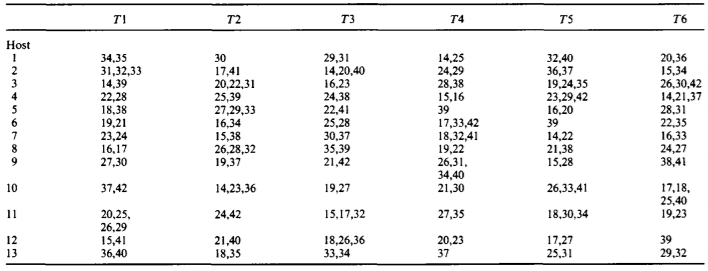
\includegraphics[width=1.0\textwidth]{party3.png}
 \caption{Solución óptima encontrada en ~\cite{Brailsford:1996:OSE:241748.241755}}
\end{figure}

Posteriormente, se eliminaron las restricciones adicionales y el programa permite buscar una solución sin esta intervención. Encontró una solución al problema de 42 yates en 27 minutos, y continuó con una solución para el siguiente período de tiempo en otro minuto, de modo que el evento podría haber durado más tiempo sin necesidad de más anfitriones.
\end{itemize}
\end{itemize}

En el paper \textit{Solving Lineal Pseudo-Boolean Constraint Problems with Local Search}~\cite{Walser:1997:SLP:1867406.1867448} se trata el problema con una búsqueda local, el cual es mucho mas eficiente que los otros modelos, pudiendo resolver el problema más rápido. Se introduce la búsqueda local de dominio independiente para satisfacibilidad (\textit{Walksat}), el cual puede generalizarse para manejar sistemas de restricciones lineales pseudo-booleanas, representación que se usa a menudo en la investigación operativa. Se introduce de esta búsqueda el algoritmo $\text{W}_{\text{SAT}}$($\mathcal{PB}$) (\textit{WalkSATisfiability}), heurística que sobre problemas de tamaño realista es eficiente para encontrar buenas soluciones aproximadas, pero su desempeño en estos problemas es a menudo críticamente dependiente de los conceptos incorporados del \textit{Tabu Search} (Como el uso de una lista \textit{Tabu Memory}).

Probando este algoritmo sobre nuestro problema obtenemos lo siguiente:
\begin{figure}[ht]
\centering
 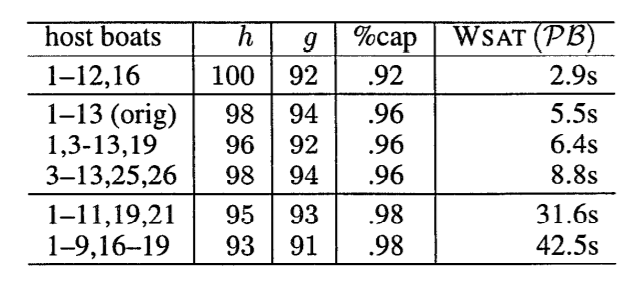
\includegraphics[width=0.6\textwidth]{party4.png}
 \caption{Comparaciones empíricas de las variaciones de PPP}
\end{figure}
\\
Donde las columnas son:

\begin{itemize}
\item \textit{host boats}: Anfitriones seleccionados.
\item \textit{h}: Suma total de las capacidades de holgura del anfitrión $h$.
\item \textit{g}: Suma total del tamaño de las tripulaciones $g$.
\item \textit{\% cap}: Porcentaje de la capacidad total usada como una medida de restricción $g$.
\item $\text{W}_{\text{SAT}}$($\mathcal{PB}$): Promedio de tiempos de ejecución sobre 20 ejecuciones de $\text{W}_{\text{SAT}}$($\mathcal{PB}$)
\end{itemize}

Cada solución con 13 anfitriones es óptima porque las limitaciones de capacidad no se pueden cumplir con 12 anfitriones, ni siquiera por un solo período de tiempo. La solución del problema se puede dividir en dos etapas: 

\begin{itemize}
    \item Selección de los barcos anfitriones.
    \item Asignación de barcos invitados a los anfitriones para todos los períodos de tiempo
\end{itemize}

Por lo que la capacidad disponible de los barcos es un buen indicador de si un barco debe ser anfitrión o invitado, de modo que después de obligar a los barcos a ser anfitriones (por ejemplo, el organizador del club), los anfitriones restantes se seleccionaron disminuyendo la capacidad libre (la capacidad disponible de un barco es su capacidad total menos el tamaño de su tripulación). El tiempo de ejecución de la instancia original descrito en ~\cite{Smith1996} es de 27 minutos, mientras que el tiempo descrito en este paper es de 8 minutos (debido a la limitación computacional de la maquina). 

En el paper \textit{Mixed logical-linear programming}~\cite{Hooker1999395} se modela el problema como un MLLP (\textit{Mixed-Logical Lineal Programming}). Se interpreta las variables multivalentes como variables numéricas y hace cumplir las restricciones totalmente diferentes. La complejidad de esto es O(B$^2$T), y la función objetivo sigue siendo encontrar la mínima cantidad de yates anfitriones.
Sin embargo, esto fue probado solo con instancias pequeñas, y con el problema completo aun sigue siendo insoluble.

Cercano al año 2000, el paper \textit{Solving the Progressive Party Problem by Local Search}~\cite{Galinier1999} nos presenta una tercera alternativa para poder resolver nuestro problema, presentando un \textit{approach} de PPP basado en Búsqueda Local. Estos resultados son mejores que los experimentos anteriores y constituyen una alternativa muy eficiente para poder resolver nuestro problema. Formulando el problema como un CSP: tomamos $T$ como el numero de periodos, $G$ como el número de botes invitados y $H$ como el numero de yates anfitriones. Además, definimos $c(g)$ para denotar el tamaño de una tripulación, donde  $g \in \{ 1,\ldots, G\}$, $C(h)$ la capacidad de un barco anfitrión donde $h \in \{ 1,\ldots H\}$ y $x_{g,t} \in \{ 1,\ldots H\}$ el yate anfitrión visitado por la tripulación g durante el periodo $T$. Como instanciación inicial tenemos H = 13 barcos anfitriones y 29 yates invitados, y la siguiente tabla nos muestra las capacidades de cada barco y el tamaño sus tripulaciones respectivas.

\begin{table}[h!]
 \centering
    \begin{tabular}{|l|l|l|l|l|}
    \hline
    Capacity C & \#boats & ~ & size c & \#crews \\ \hline
    10         & 2       & ~ & 7      & 1       \\
    9          & 1       & ~ & 6      & 1       \\
    8          & 6       & ~ & 5      & 3       \\
    7          & 1       & ~ & 4      & 8       \\
    6          & 1       & ~ & 3      & 2       \\
    4          & 1       & ~ & 2      & 14      \\ \hline
    ~          & 13      & ~ & ~      & 29      \\ \hline
    \end{tabular}
\end{table}

Tenga en cuenta, sin embargo, que un límite superior obvio para T es 10. De hecho, hay un equipo de invitados de tamaño 7 y sólo 10 \textit{hosts} tienen una capacidad mayor o igual a 7. Por lo tanto, sólo 10 \textit{hosts} pueden ser asignados a esta tripulación de invitados con el fin de respetar la limitación de capacidad. Por otra parte, esta tripulación de invitados debe visitar un anfitrión diferente en cada período de tiempo. Por lo tanto, el número de períodos de tiempo no puede exceder de 10. Las restricciones definidas son: 

\begin{itemize}
    \item El primer tipo de restricciones impone que cada tripulación se mueva a un anfitrión diferente en cada período de tiempo, la cual se denominan DIFF($g$),
    \item El segundo tipo de restricciones impone que dos tripulaciones se reúnan a lo sumo una vez: para cada par de tripulaciones invitadas, el número de periodos de tiempo en que se reúnen estas dos tripulaciones es 0 o 1. Se denomina como ONCE(\{$g1,g2$\}).
    \item El tercer tipo de restricciones impone que se respete la capacidad de los barcos anfitriones. Se denomina como CAPA ($h,t$). 
\end{itemize}

las cuales son similares al modelo CSP de ~\cite{Smith1996}. 
Como se ha expuesto anteriormente, una configuración es una asignación completa de los números en $D = {1,\ldots ,H = 13}$ a las variables de $X = {x_{gt}, 1 \leq g \leq G, 1 \leq t \leq T}$: a La configuración es una tabla $G x T (G = 29 y T = 6,7,8,9 o 10)$ cuyos elementos son números enteros de $\{1\ldots 13\}$. El espacio de búsqueda es el conjunto de todas estas asignaciones. Además, se plantea una función de costos, la cual se define como el número de restricciones violadas,asociando a cada restricción $C$ una penalidad $f_C (s)$ que toma 1 o 0 según que la restricción sea violada o no. De hecho, esta función no puede distinguir una restricción "fuertemente violada" de una "débilmente" violada. En el PPP, las restricciones son más complejas, por lo que se proponen una función de \textit{penalty} para las restricciones ~\cite{Galinier1999}. Luego, la Finalmente la función de costo (evaluación) nos queda de la siguiente forma:
\begin{align*}
  \displaystyle \sum_{C \in \mathcal{C}} p(\mathit{C}) * f_{C}(s)
\end{align*}

Donde $p$ es el peso de la cada función. 
Las mejores ponderaciones encontradas son 4, 2 y 4 para DIFF, ONCE y CAPA respectivamente.

Luego, definimos dos tipos de movimientos:
\begin{itemize}
    \item \textit{OneMove}: \\
    Un movimiento del tipo OneMove consiste simplemente en cambiar el barco anfitrión afectado a una tripulación dada por un período dado, es decir, el valor actual de una sola variable $x$ es reemplazado por uno nuevo $v$.
    
    \item \textit{Swap}: \\
    Un cambio de \textit{swap} consiste en invertir los barcos anfitriones asignados a dos tripulacion $g_1$ y $g_2$ durante el mismo periodo de tiempo $t$. 
\end{itemize}

Teniendo esto, se definen 2 principales tipos de meta-heurísticas: \textit{Metropolis algorithm} y {Tabu Search algorithm}. 

\begin{itemize}
 \item \textbf{\textit{Metropolis algorithm}}: \\
 El algoritmo Metrópolis es una versión simplificada de \textit{Simulated Annealing} que utiliza un valor constante para su parámetro de temperatura. El algoritmo comienza con una configuración inicial en el espacio de búsqueda y luego realiza una serie de iteraciones. En cada iteración, se elige aleatoriamente un solo vecino (o equivalentemente un solo movimiento) de la configuración actual y luego se realiza un criterio probabilístico para decidir si este vecino es aceptado o no. El principio del algoritmo Metrópolis es aceptar cualquier movimiento que no aumente la función de coste, y aceptar, de manera controlada, movimientos de deterioro. Así se asegura de que el algoritmo no quede atrapado en un óptima local.
 
El método tiene un parámetro $\theta$ llamado temperatura: cuanto más alto es el valor de la temperatura, se aceptan las degradaciones más fáciles (una temperatura cero corresponde a un descenso ya que todos los movimientos de deterioro son rechazados mientras que una temperatura infinita es realizar muchos cambios aleatorios en el espacio de búsqueda, ya que todos los movimientos son aceptados).

\item \textbf{\textit{Tabu search}}: \\
El algoritmo búsqueda de tabú comienza con una configuración inicial en el espacio de búsqueda y luego procede iterativamente a visitar una serie de configuraciones localmente mejores siguiendo el vecindario. En cada iteración, se aplica un mejor movimiento a la configuración actual , incluso si la solución no mejora la configuración actual en términos del valor de la función de coste. 

Este proceso iterativo puede sufrir ciclismo y quedar atrapado en un óptimo local. Para evitar este problema, TS introduce la noción de listas Tabú. Una lista tabú es una lista especial de corto plazo que mantiene un historial, compuesta de soluciones previamente encontradas. Una estrategia de TS simple basada en esta lista de corto plazo consiste en evitar que las soluciones guardadas sean reconsideradas para próximas k iteraciones (k, denominada tenencia de tabú, depende del problema). 

En la siguiente tabla se presentan los resultados computacionales de diferentes modelos

\end{itemize}



\section{Modelo Matemático}
Se presenta la primera formulacion del problema \textit{Progressive Party Problem }, descrito de la siguiente manera:

\begin{itemize}
    \item Variables:
    \begin{itemize}
        \item $h_i$: 1 si el yate $i$ es un yate anfitrión
        \item $x_{ikt}$: 1 si el yate $k$ es un invitado del yate $i$ en el periodo $t$. (El dueño del yate organizador del club esta restringido a ser anfitrión en todos los modelos).
        \item $m_{klt}$: 1 si la tripulación $k$ y la tripulación $l$ se encuentran en el periodo $t$.
    \end{itemize}
    \item Función objetivo:
    \begin{itemize}
        \item Minimizar $\displaystyle \sum_{i} h_i$
    \end{itemize}
    \item Restricciones:
    \begin{align}
        \displaystyle x_{ikt} - h_i &\leq 0           & \text{para todo } i,k,t;i\neq k  \\ 
        \displaystyle \sum_{k,k\neq i} c_k x_{ikt} & \leq g_i & \text{para todo } i,t \\
        & & \text{ donde } g_i  \text{: max} \{K_i - c_i,0 \} \\
        \displaystyle \sum_{i,i\neq k} x_{ikt} + h_k &= 1            & \text{para todo }k,t \\
        \displaystyle \sum_{t} x_{ikt} &\leq 1            & \text{para todo } i,k;i \leq k \\
        \displaystyle m_{klt} &\geq x_{ikt} + x_{ilt} -1           & \text{para todo } k,l,t; k<l \\
        \displaystyle \sum_{t} m_{klt} &\leq 1 & \text{para todo } k,l,t; k<l
    \end{align}
    Sobre las restricciones:
    \begin{itemize}
        \item (1) Un bote solo puede ser visitado si es un yate anfitrión.
        \item (2) La capacidad de un yate anfitrión no puede ser excedida. Además, $c_i$ es el tamaño de la tripulación del bote $i$ y $K_i$ es la capacidad total del yate.
        \item (3) Cada tripulación debe tener al menos un yate anfitrión.
        \item (4) Una tripulación no puede visitar un yate anfitrión mas de una vez. 
        \item (5) y (6): Como el barco anfitrión i es irrelevante, la siguiente formulación es más apropiada que en ~\cite{Walser:1997:SLP:1867406.1867448}. Se define la variable binarias $m_{klt}$ en lugar de $y_{iklt}$ que toma el valor 1 si las tripulaciones k y l se reúnen en el instante t. Si no se reúnen entonces, dejamos $m_{klt}$ sin restricciones.
    \end{itemize}
\end{itemize}

Se propone un segundo modelo como CSP, la cual es un poco mas compacta. Supongamos que tenemos $G$ barcos invitados, $H$ yates \textit{host} y $T$ periodos:
\begin{itemize}
    \item Variable:
    \begin{itemize}
        \item $h_{it}$: Yate anfitrión que el yate invitado $i$ visito en el periodo $t$.
        \item Dominio $h_{it}$: $\{1,\ldots H \}$, con un total de $GT$ variables.
    \end{itemize}
    \item Restricciones:
    \begin{itemize}
        \item La restricción de que cada barco invitado debe tener siempre un anfitrión y que en cualquier período de tiempo un barco invitado sólo puede ser asignado a un \textit{host} son automáticamente satisfechas por cualquier solución del CSP, donde exactamente se asigna un anfitrión a cada barco invitado en cada período de tiempo.
        \item La restricción de que ningún barco invitado puede visitar un barco anfitrión más de una vez en el modelo CSP se expresa como:
        \begin{align*}
            &h_{i1},h_{i2},h_{i3},\ldots h_{iT} \text{ sean todos distintos para todo } i\neq k \\
            &h_{i1} \neq h_{i2}, \ldots 
        \end{align*}
        Donde para cada $i$, esto no es mas que una restricción de tipo \textit{Solve} para el problema, quedando $\displaystyle\frac{T(T-1)}{2}$  restricciones binarias desiguales.
        \item Las restricciones de capacidad son tratadas como en LP:
        \begin{align*}
            v_{ijt} = 1 \text{ si y solo si } h_{it} = j, \text{ para todo } i,j,t.
        \end{align*}
        Donde la relacion entre $v_{ijt}$ y $h_{it}$ es de GHT variables booleanas. Finalmente la restricción de capacidad nos queda como:
        \begin{align*}
            \sum_{i} c_{i}v_{ijt} \leq C_j, \text{ para todo } j,t.
        \end{align*}
        
        Donde $c_i$ es el tamaño de la tripulación de invitado barco $i$ y $C_j$ es la capacidad de reserva del barco anfitrión $j$, después de acomodar a su propia tripulación.
        
        \item La restricción de que ningún par de tripulaciones pueda encontrarse dos veces también requiere de una nueva variable binaria:
        \begin{align*}
            \text{si } h_{kt} = h_{lt} \text{ entonces } m_{klt} = 1, \text{ para todo } k,l,t; k<l.
        \end{align*}
        Por lo tanto la restricción de encuentro queda como:
        \begin{align*}
            \sum_{t} m_{klt} \leq 1 ,\text{ para todo } k,l;k<l
        \end{align*}
    \end{itemize}
\end{itemize}


\section{Conclusiones}
Conclusiones RELEVANTES del estudio realizado. Deber\'ia responder a las preguntas: ?`todas las t\'ecnicas resuelven el mismo problema o hay algunas diferencias?, ?`En qu\'e se parecen o difieren las t\'ecnicas en el contexto del problema?, ?`qu\'e limitaciones tienen?, ?`qu\'e t\'ecnicas o estrategias son las m\'as prometedoras?, ?`existe trabajo futuro por realizar?, ?`qu\'e ideas usted propone como lineamientos para continuar con investigaciones futuras?


\section{Bibliograf\'ia}
Indicando toda la informaci\'on necesaria de acuerdo al tipo de documento revisado. Todas las referencias deben ser citadas en el documento.
\bibliographystyle{plain}
\bibliography{Referencias}

\end{document} 